\documentclass[11pt]{article}
\usepackage[T1]{fontenc}
\usepackage[utf8]{inputenc}
\usepackage{lmodern}
\usepackage[margin=1in]{geometry}
\usepackage{amsmath,amssymb,amsthm,mathtools}
\usepackage{microtype,booktabs,array,longtable,enumitem}
\usepackage{graphicx}
\usepackage[hidelinks]{hyperref}
\usepackage{xurl}
\usepackage{fancyhdr}
\hypersetup{pdftitle={Sharp Weighted Four-State Hierarchy Prices for Polynomial Curvature},pdfauthor={Wenyu Huang},pdfsubject={Phase 9 follow-up working paper},pdfkeywords={Bregman divergence, hierarchy price, polynomial curvature, positive weights, proper loss}}
\setlength{\headheight}{14pt}
\pagestyle{fancy}\fancyhf{}
\fancyhead[L]{\small Sharp weighted four-state hierarchy prices}
\fancyhead[R]{\small Phase 9}
\fancyfoot[C]{\thepage}
\setlength{\parskip}{0.25em}
\setlength{\emergencystretch}{2em}
\renewcommand{\arraystretch}{1.15}
\newtheorem{theorem}{Theorem}[section]
\newtheorem{lemma}[theorem]{Lemma}
\newtheorem{proposition}[theorem]{Proposition}
\newtheorem{corollary}[theorem]{Corollary}
\theoremstyle{definition}\newtheorem{definition}[theorem]{Definition}
\theoremstyle{remark}\newtheorem{remark}[theorem]{Remark}
\newcommand{\ph}{\varphi}
\newcommand{\B}{B_{\ph}}
\newcommand{\D}{D_{\ph}}
\newcommand{\OPT}{\operatorname{OPT}}
\newcommand{\E}{\mathbb E}
\newcommand{\R}{\mathbb R}
\newcommand{\rd}{\,\mathrm d}
\newcommand{\detp}{\mathrm{det}}
\newcommand{\stp}{\mathrm{stoch}}
\title{Sharp Weighted Four-State Hierarchy Prices\\ for Polynomial Curvature}
\author{Wenyu Huang\\\small University of California San Diego}
\date{Phase 9 follow-up working paper\\7 October 2026}
\begin{document}
\maketitle
\begin{center}\begin{minipage}{0.92\textwidth}\small
\textbf{Status.} The mathematical arguments received internal independent
review. This is not external peer review or formal verification. Historical
originality has not been established, and no priority claim is made.
\end{minipage}\end{center}

\begin{abstract}
We determine the degree order of optimal two-/three-capacity hierarchy
prices on four weighted source states. For nonnegative polynomial curvature
of degree at most $r$, with arbitrary positive probabilities and posterior
locations, the deterministic and stochastic worst-case prices are both
$\Theta(r^2/(\log r)^2)$. The upper bound is explicitly
$1936r^2/(\log r)^2$ for $r\ge2$. Its proof selects a weighted triple using
the two middle masses, compares its exact Jensen kernel with the outer-pair
kernel, and combines classical Markov and Chebyshev inequalities. A full
endpoint lower construction from the preceding working paper is reproduced.
Separately, the classical coordinate $h=\int\sqrt{\varphi''}$ has unavoidable
two-sided partition-comparison distortion $\Omega(r^2\log r)$ for one
strictly positive polynomial and one three-state source whose actual
all-capacity hierarchy price is one. This limits that comparison method,
not the optimal hierarchy. We also give an exact oracle equivalence for
restricted indicator-ReLU splitting and show why unrestricted neuron count
does not inherit it. Classical Jacobi endpoint moments identify sharp
oriented Bregman asymmetry in an appendix. Arbitrary-source-count degree
orders, learning guarantees, and nonvanishing absolute-risk separations
remain outside the conclusions.
\end{abstract}

\section{The four-state problem and the result}
Separately optimal finite representations can be incompatible: an optimal
three-cell partition need not refine an optimal two-cell partition.
Under a strictly proper binary loss, the excess Bayes risk of a
representation is a scalar Jensen distortion. Its hierarchy price is the
smallest simultaneous multiplicative factor when the two-cell
representation must be obtained by coarsening the three-cell one.

The preceding Phase~8 working paper~\cite{huang8} established a sharp
$\Theta(r/\log r)$ degree envelope for four equal source masses and an
$\Omega(r^2/(\log r)^2)$ lower bound when positive masses and posterior gaps
may vary with degree. Its general two-capacity upper bound was $O(r^2)$.
The present paper closes this logarithmic gap for exactly four states:
if $\widehat C_r^{\detp}$ and $\widehat C_r^{\stp}$ denote the
arbitrary-positive-weight four-state envelopes, then, for an absolute
$c>0$ and all sufficiently large $r$,
\begin{equation}
 c\frac{r^2}{(\log r)^2}
 \le \widehat C_r^{\stp}\le\widehat C_r^{\detp}
 \le1936\frac{r^2}{(\log r)^2}.
 \label{eq:main-envelope}
\end{equation}
All logarithms are natural, and $r$ is the degree of the curvature
$\varphi''$, not of the generator $\varphi$.

The upper proof retains the original source masses in every cell kernel.
An isolated weighted triple cannot support the required degree inference:
even constant curvature gives a counterexample to the naive pair of
three-point cost inequalities. The successful argument chooses between
the two adjacent triples using their common middle masses. It then replaces
the selected triple kernel by its outer-pair kernel, with error controlled
by the two adjacent costs. This permits a nearby polynomial peak to force
enough curvature mass in the middle-pair interval. The explicit estimate is
\[
 R^2\le16r^2e^{20r/\sqrt R}\qquad(R\ge128),
\]
where $R$ is the actual deterministic price. No lower bound on a source
mass or posterior gap appears in the constants.

\begin{table}[ht]
\centering\small
\begin{tabular}{@{}>{\raggedright\arraybackslash}p{0.30\textwidth}>{\raggedright\arraybackslash}p{0.31\textwidth}>{\raggedright\arraybackslash}p{0.31\textwidth}@{}}
\toprule
Domain & Established degree order or bound & Status in this paper\\
\midrule
Four states; arbitrary positive weights; capacities two and three
& $\Theta(r^2/(\log r)^2)$ in both models
& Sharp order; full upper and lower proofs\\
Four states; all capacities
& Same price as capacities two and three
& One and four outputs add no cost\\
Arbitrary finite source count; two prescribed capacities
& Prior upper $1+128r^2$; lower $\Omega(r^2/(\log r)^2)$ witnessed at $(2,3)$
& General degree order remains open\\
Arbitrary finite source count; all capacities
& Prior upper $256r^2K_r$; same lower, where $K_r=2\log(64r^2)+1/4$
& General degree order remains open\\
One source and the coordinate $h=\int\sqrt g$
& Comparison condition factor $\Omega(r^2\log r)$
& Method obstruction; example has hierarchy price one\\
\bottomrule
\end{tabular}
\caption{Distinct quantifiers. The general-source upper bounds are prior
Phase~8 results, not new consequences of the four-state proof. Upper
statements also bound stochastic prices; lower statements apply to both
models.}
\label{tab:scope}
\end{table}

Two further points prevent overinterpretation. First, a comparison of
Bregman costs with squared distances may be much worse than the hierarchy
itself. Section~\ref{sec:coordinate} realizes both sharp comparison losses
for the same positive polynomial and the same three-state source. Second,
an exact partition model can be embedded in a restricted indicator-ReLU
class, but an unrestricted single ReLU already fits every posterior on the
same one-hot domain. Section~\ref{sec:p9-indicator-bridge} therefore states
an oracle equivalence with its constraints, rather than a neural-width or
training theorem.

\paragraph{Relation to classical tools and prior work.}
Bregman centroids and proper-loss regret identities are classical
\cite{banerjee,gneiting,reid}. Hierarchical clustering approximation has
an established literature, including Lin et al.~\cite{lin} and
Arutyunova--R\"oglin~\cite{arutyunova}. The present four-state upper proof
does not invoke a general hierarchy-augmentation theorem. Its polynomial
ingredients are classical Markov and Chebyshev inequalities
\cite{shadrin,dlmf}. Explicit squared-Chebyshev endpoint needles and
$\exp(-c r\sqrt d)$ endpoint tails occur in Slot--Laurent
\cite[Section~4.1]{slot2019}, with earlier attribution there; related
$O(\log^2 r/r^2)$ approximation bounds appear in~\cite{slot2020}.
The endpoint lower proof below supplies its own normalization and weighted
kernel estimates and does not claim the needle construction as new.

The exact Jacobi first-moment calculation in Appendix~\ref{sec:p9-exact-asymmetry}
is a classical positive-quadrature consequence, with a direct antecedent in
de Klerk--Laurent~\cite{deklerk} and related spectral formulations in
Lasserre~\cite{lasserre}. These approximation problems do not establish
partition incompatibility or the hierarchy order in~\eqref{eq:main-envelope}.
The focused source check is bounded, not an exhaustive originality review.

\section{Distortion, channels, and hierarchy prices}
\label{sec:definitions}
Let a source index $X$ take values in $\{1,\ldots,N\}$ with probabilities
$p_i>0$, $\sum_i p_i=1$, and posterior locations $x_i\in[0,1]$.
Unless stated otherwise, $\varphi$ is differentiable and strictly convex.
For polynomial results it is $C^2$ with nonnegative, nonzero polynomial
curvature $g=\varphi''$. Such a polynomial vanishes on no nonempty
interval, so $\varphi$ is strictly convex even when $g$ has isolated zeros.
The oriented Bregman divergence is
\[
 B_\varphi(x,y)=\varphi(x)-\varphi(y)-\varphi'(y)(x-y).
\]
For a partition $P$, set
\begin{equation}
 D_\varphi(P)=\sum_{C\in P}D_\varphi(C),\qquad
 D_\varphi(C)=\sum_{i\in C}p_i\varphi(x_i)-p_C\varphi(m_C),
 \quad p_C=\sum_{i\in C}p_i,
 \quad m_C=\frac{\sum_{i\in C}p_ix_i}{p_C}.
 \label{eq:distortion}
\end{equation}
Cell costs always use original source probabilities, without conditional
renormalization. Write $D(AB)$ for the cost of the cell containing states
$A,B$, and similarly for larger cells. The flat optimum $\OPT_k$ is the
minimum of $D_\varphi(P)$ over partitions with at most $k$ cells.
Refinement never increases distortion.

\begin{lemma}[Centroids and curvature kernels]
\label{lem:identities}
For every cell $C$ and report $q\in[0,1]$,
\begin{equation}
 \sum_{i\in C}p_iB_\varphi(x_i,q)
 =D_\varphi(C)+p_CB_\varphi(m_C,q).
 \label{eq:centroid}
\end{equation}
For $u<v$ the two orientations are
\[
 B_\varphi(v,u)=\int_u^v(v-t)g(t)\,dt,
 \qquad B_\varphi(u,v)=\int_u^v(t-u)g(t)\,dt.
\]
Moreover $D_\varphi(C)=\int_0^1 K_C(t)g(t)\,dt$, where
\begin{equation}
 K_C(t)=\sum_{i\in C}p_i(x_i-t)_+-p_C(m_C-t)_+\ge0.
 \label{eq:kernel}
\end{equation}
\end{lemma}
\begin{proof}
Expand the Bregman expression and use
$\sum_{i\in C}p_i(x_i-m_C)=0$ to obtain~\eqref{eq:centroid}.
Twice integrating $g$ gives the two orientation formulas and the identity
$\varphi(x)=\varphi(0)+\varphi'(0)x+
\int_0^1(x-t)_+g(t)\,dt$. Affine terms cancel in a Jensen gap,
giving~\eqref{eq:kernel}. Its nonnegativity is Jensen's inequality for
the convex hinge $x\mapsto(x-t)_+$.
\end{proof}

A deterministic hierarchy at capacities $k<\ell$ is a pair of partitions
$H_\ell\succeq H_k$, where $\succeq$ denotes refinement and
$|H_j|\le j$. When both flat denominators are positive, its price is
$\max_{j\in\{k,\ell\}}D_\varphi(H_j)/\OPT_j$.
The minimum over all such pairs is $\rho_{\varphi,\detp}$.
Unless specified otherwise, four-state prices use $k=2,\ell=3$.
There is no restriction that a hierarchical cell be contiguous in the
ordered posterior locations.

For a channel $X\to Z$, define
\[
 D_\varphi(Z)=\E\varphi(x_X)-
                \E\varphi\bigl(\E[x_X\mid Z]\bigr).
\]
A stochastic hierarchy is a degradation chain
$X\to Z_\ell\to Z_k$, with $|Z_j|\le j$; its optimal price
$\rho_{\varphi,\stp}$ is the infimum of the same maximum ratio.
The predictor is not supplied an additional public random seed.

\begin{lemma}[The stochastic and deterministic flat optima coincide]
\label{lem:flat}
The infimum of $D_\varphi(Z)$ over channels with at most $k$ outputs is
$\OPT_k$.
\end{lemma}
\begin{proof}
Realize any channel by a random function table $U$, independent of $X$:
for each input draw one output according to that channel row. Conditional
on $U$, the map is deterministic and has at most $k$ outputs. Conditional
Jensen implies
\[
 \E\varphi(\E[x_X\mid Z])\le
 \E\varphi(\E[x_X\mid Z,U]).
\]
Thus $D_\varphi(Z)\ge\E_U D_\varphi(Z\mid U)\ge\OPT_k$.
A deterministic minimizer gives the reverse inequality.
\end{proof}

\begin{lemma}[Two-level deterministic comparison]
\label{lem:ext-rounding}
For any finite source, strictly convex generator, and two output capacities
with positive flat distortions,
\[
 \tfrac12\rho_{\ph,\detp}\le\rho_{\ph,\stp}
 \le\rho_{\ph,\detp}.
\]
\end{lemma}
\begin{proof}
For a stochastic degradation chain, sample independent deterministic function
tables for its encoder and coarsener, independently of the source, and call
the pair of tables $U$. Conditional on $U$ the two representations form an
admissible deterministic hierarchy. Revealing $U$ can only reduce Jensen
distortion, so at each of the two levels $k$,
\[
 D(Z_k)\ge\mathbb E_U D(Z_k\mid U).
\]
Let $R$ be the price of this particular stochastic chain. The expected sum of
the two deterministic conditional ratios is at most $2R$. At least one table
therefore has sum at most $2R$, and its maximum ratio is no larger than its
sum. Consequently $\rho_{\ph,\detp}\le2R$; take the infimum over chains.
Deterministic chains are themselves admissible stochastic chains, proving the
other direction. No public random seed is available to the actual predictor;
revealing the tables is used only in this proof.
\end{proof}



An all-capacity deterministic hierarchy has $H_{k+1}\succeq H_k$ and
$|H_k|\le k$ for $1\le k\le N$; the stochastic version is a chain
$X\to Z_N\to\cdots\to Z_1$. At zero optima we use the cost-inequality
definition: the price is the smallest factor $c$ for which
$D_\varphi(H_k)\le c\OPT_k$ at every capacity, and likewise for channels.
In particular a zero optimum requires zero hierarchical cost. On four
states, any two-/three-capacity hierarchy extends by a constant output at
capacity one and the identity at capacity four, so its all-capacity price
is unchanged, in either model.

For an integer $r\ge0$, define $\widehat C_r^{\detp}$ and
$\widehat C_r^{\stp}$ as the suprema of these four-state two-/three-capacity
prices over all positive probability vectors, all locations in $[0,1]$
with $\OPT_2,\OPT_3>0$, and all generators with nonnegative, nonzero
polynomial curvature of degree at most $r$. The generator, masses, and
locations may all vary with $r$. Multiplying $\varphi$ by a positive
constant scales all distortions equally and preserves every price;
adding an affine function preserves the distortions themselves.

% Phase 9 research candidate; include-ready for curvature_hierarchy.tex.
% All Phase 8 source files are immutable and were only read.
% Independently checked algebraically by endpoint_obstruction and
% phase9_adversarial on 7 October 2026. Internal review only.
\section{The sharp degree order for four arbitrary positive weights}
\label{sec:weighted-sharp}

The four-state arbitrary-weight degree envelope has the sharp order
announced in the introduction. The proof uses the original source weights
in every Jensen kernel. Choosing the appropriate one of the two adjacent
triples is essential: a corresponding assertion for an arbitrary weighted
triple would be false.

\begin{theorem}[Weighted four-state degree bound]
\label{thm:weighted-sharp}
Let $g=\varphi''$ be a nonzero polynomial of degree at most $r$, nonnegative
on $[0,1]$. Let four source states have arbitrary positive probabilities
and posterior locations in $[0,1]$, and suppose that both flat distortions
$\operatorname{OPT}_2$ and $\operatorname{OPT}_3$ are positive. Write
$R=\rho_{\varphi,\mathrm{det}}$ for the optimal deterministic hierarchy
price at output budgets two and three.
If $r\ge1$ and $R\ge128$, then
\begin{equation}
 R^2\le16r^2\exp\left(\frac{20r}{\sqrt R}\right).
 \label{eq:weighted-implicit}
\end{equation}
In particular, if $R\ge256$ then
\begin{equation}
 R(\log R)^2\le1936r^2.
 \label{eq:weighted-Rlog}
\end{equation}
For every integer $r\ge2$ this gives the explicit uniform bound
\begin{equation}
 \rho_{\varphi,\mathrm{stoch}}
 \le\rho_{\varphi,\mathrm{det}}
 \le1936\frac{r^2}{(\log r)^2}.
 \label{eq:weighted-sharp-upper}
\end{equation}
Consequently, in the four-state degree envelopes permitting all positive
weights and all posterior locations, both prices have sharp order
\[
 \widehat C_r^{\mathrm{det}}
 =\Theta\!\left(\frac{r^2}{(\log r)^2}\right),\qquad
 \widehat C_r^{\mathrm{stoch}}
 =\Theta\!\left(\frac{r^2}{(\log r)^2}\right).
\]
The matching lower bounds follow from the endpoint construction, reproduced in
Theorem~\ref{thm:ext-weightdegenerate}.
\end{theorem}

\begin{proof}
We first record the two elementary polynomial estimates used below. If
$f\ge0$ is a polynomial of degree at most $r\ge1$ on an interval $E$ of
length $L>0$, and $M_E=\max_E f$, then the rescaled Markov inequality~\cite{shadrin} gives
\begin{equation}
 \int_E f(t)\,\mathrm dt\ge\frac{L M_E}{8r^2}.
 \label{eq:weighted-markov-mass}
\end{equation}
Indeed, $\|f'\|_\infty\le2r^2M_E/L$. From a maximizer there is an
available one-sided segment of length $L/(4r^2)$, and on this segment
$f\ge M_E/2$.

If $t_0$ lies to the right of $E$, at distance $d$ from its right endpoint,
the classical Chebyshev extremal inequality gives
\begin{equation}
 |f(t_0)|\le M_E T_r(1+2d/L)
 \le M_E\exp\left(2r\sqrt{d/L}\right).
 \label{eq:weighted-cheb-extrapolation}
\end{equation}
Here the second estimate follows from
$T_r(\cosh s)=\cosh(rs)$ and
$\operatorname{arcosh}(1+x)\le\sqrt{2x}$. To see the first estimate
directly, rescale $E$ to $[-1,1]$ and divide by $M_E$. If a degree-at-most-$r$
polynomial $F$ bounded by one there had
$|F(z)|>T_r(z)$ at $z>1$, change its sign if necessary and set
$\lambda=T_r(z)/F(z)\in(0,1)$. At the $r+1$ alternating extrema of $T_r$,
the polynomial $T_r-\lambda F$ has the same strict alternating signs as
$T_r$, giving $r$ roots in $[-1,1]$, as well as its root at $z$.
This contradicts its degree. These estimates are classical polynomial
tools, not new approximation results.

\emph{The sole optimizer conflict is still the middle pair.}
Positive $\operatorname{OPT}_3$ implies that the four posteriors are
distinct; label them $A<B<C<D$. For a cell or pair, retain its original
source weights without conditional renormalization. Put
\[
 p_L=D(AB),\quad q=D(BC),\quad p_R=D(CD),\quad
 Q=p_L+p_R,\quad T_L=D(ABC),\quad T_R=D(BCD).
\]
Contiguous flat optimizers exist for arbitrary positive weights: for fixed
centers $a<b$, the difference $B_\varphi(x,a)-B_\varphi(x,b)$ is affine
in $x$ with positive slope, so nearest-center assignments are contiguous,
and updating to weighted centroids cannot increase distortion. Strict
convexity and distinct posteriors ensure that the optimum fills its budget.

For every weighted triple, its kernel dominates the two constituent
adjacent-pair kernels on their respective disjoint interiors. One way to
see the domination is to merge a pair first and then merge its weighted
centroid with the remaining state; the additional Jensen gap is
nonnegative, including for each hinge generator. Thus
\[
 T_L\ge p_L+q,\qquad T_R\ge q+p_R.
\]
If $AB$ is a cheapest adjacent pair, the only incompatible contiguous
coarse candidate is $A\mid BCD$; its cost obeys
$T_R\ge q+p_R\ge p_L+p_R=Q$, so a compatible flat-optimal coarse
partition can be chosen. The case of $CD$ is its reflection. If $BC$ is
cheapest and either triple split is flat optimal, it too has compatible
flat optima. Hence either $R=1$, or we may work with the sole conflict
\[
 \operatorname{OPT}_3=q,\qquad \operatorname{OPT}_2=Q,
\]
where the optimal fine pair is $BC$ and the optimal coarse split is
$AB\mid CD$.

The hierarchy retaining that coarse split and its cheaper outer fine pair,
and the two hierarchies retaining the fine pair $BC$ and an adjacent triple,
give the admissible-candidate inequalities
\begin{equation}
 R\le\frac{\min(p_L,p_R)}q,\qquad
 R\le\frac{T_L}Q,\qquad R\le\frac{T_R}Q.
 \label{eq:weighted-candidates}
\end{equation}
They use feasible deterministic hierarchies only. They do not require an
exhaustion of optimal noncontiguous hierarchies.

\emph{Choose the triple by the middle masses.}
Reflect the ordered configuration if necessary so that $p_B\le p_C$.
Use the triple $BCD$, and affinely normalize its own hull to $[0,1]$:
\[
 B=0,\quad C=c\in(0,1),\quad D=1,\qquad
 (p_B,p_C,p_D)=(u,v,w),\quad 0<u\le v,\quad w>0.
\]
The fourth point is not used in the polynomial estimates. If the original
triple hull has length $L_0$, the transformed curvature is
$L_0^2g(B+L_0t)$, preserving the curvature degree, nonnegativity, and all
the costs under discussion. Denote it again by $g$.

Let $K$ be the triple kernel, let $k_q$ and $k_p$ be its two adjacent-pair
kernels, and let $H$ be the kernel of its two outer states with their
original weights:
\begin{align*}
 K(t)&=\min\{ut+v(t-c)_+,\ w(1-t)+v(c-t)_+\},\\
 k_q(t)&=\min\{ut,v(c-t)\}\,\mathbf1_{[0,c]}(t),\\
 k_p(t)&=\min\{v(t-c),w(1-t)\}\,\mathbf1_{[c,1]}(t),\\
 H(t)&=\min\{ut,w(1-t)\}.
\end{align*}
In particular $T:=T_R=\int_0^1Kg$, $q=\int_0^1k_qg$, and
$p_R=\int_0^1k_pg$. Write $S=p_R+q$.
By \eqref{eq:weighted-candidates},
\begin{equation}
 q\le\frac{Q}{2R}\le\frac{T}{2R^2},\qquad
 S\le Q+q\le\frac{T}{R}+\frac{T}{2R^2}\le\frac{2T}{R}.
 \label{eq:weighted-two-small-costs}
\end{equation}

Two pointwise facts make these estimates uniform in the weights. First,
\begin{equation}
 0\le K-H\le k_q+k_p.
 \label{eq:weighted-H-comparison}
\end{equation}
For $t<c$, the difference is
$\min\{ut,w(1-t)+v(c-t)\}-\min\{ut,w(1-t)\}$,
which lies between zero and $\min\{ut,v(c-t)\}=k_q(t)$.
For $t>c$, interchange the two sides to obtain the bound by $k_p(t)$.
Second, for $t<c$, $K(t)\le ut$ gives
\[
 \frac{k_q(t)}{K(t)}
 \ge\min\left\{1,\frac{v(c-t)}{ut}\right\}
 \ge\min\left\{1,\frac{c-t}{t}\right\}.
\]
For $t>c$, put $\Delta=t-c$. The elementary inequality
$\min\{B,C\}/\min\{A+B,C\}\ge B/(A+B)$, for positive
$A,B,C$, gives
\[
 \frac{k_p(t)}{K(t)}
 \ge\frac{v\Delta}{ut+v\Delta}
 \ge\frac{\Delta}{c+2\Delta}.
\]
Endpoint values follow by continuity; ratios need only be used inside
$(0,1)$, where $K>0$.

\emph{A large peak and a nearby interval with small curvature cost.}
Assume $R\ge128$ and put
\[
 \varepsilon=\frac{16}{R}\le\frac18,
 \qquad I=\{t\in[0,1]:|t-c|\le\varepsilon c\}.
\]
The preceding pointwise inequalities imply, outside $I$,
\[
 k_q+k_p\ge\frac{\varepsilon}{1+2\varepsilon}K.
\]
Consequently
\[
 \int_{[0,1]\setminus I}Kg
 \le\frac{1+2\varepsilon}{\varepsilon}S
 \le\frac{5T}{32}.
\]
By \eqref{eq:weighted-H-comparison} and
\eqref{eq:weighted-two-small-costs},
\[
 \int_I Hg\ge T-\frac{5T}{32}-S
 \ge\frac{53T}{64}\ge\frac{3T}{4}.
\]
On $I$, $H(t)\le ut\le u(1+\varepsilon)c$, and $|I|\le2\varepsilon c$.
Thus there exists $t_0\in I$ such that
\begin{equation}
 g(t_0)\ge\frac{T}{4\varepsilon u c^2}.
 \label{eq:weighted-peak}
\end{equation}
This estimate uses $H\le ut$, rather than dividing by $H(c)$, which could
be arbitrarily small as weights or gaps degenerate.

Consider the interval
\[
 E=[c/4,c(1-2\varepsilon)].
\]
Its length is at least $c/2$. The point $t_0$ lies to its right at distance
at most $3\varepsilon c$. On all of $E$, both terms in
$k_q(t)=\min\{ut,v(c-t)\}$ are at least $2u\varepsilon c$:
indeed $t\ge c/4\ge2\varepsilon c$, $c-t\ge2\varepsilon c$, and
$v\ge u$. With $M_E=\max_Eg$, the extrapolation estimate
\eqref{eq:weighted-cheb-extrapolation} and \eqref{eq:weighted-peak} give
\[
 M_E\ge g(t_0)\exp(-\sqrt{24}\,r\sqrt\varepsilon)
 \ge\frac{T}{4\varepsilon u c^2}
       \exp\left(-\frac{20r}{\sqrt R}\right),
\]
where $4\sqrt{24}<20$. The mass estimate
\eqref{eq:weighted-markov-mass} now yields
\begin{align*}
 q&\ge2u\varepsilon c\int_Eg(t)\,\mathrm dt\\
  &\ge2u\varepsilon c\frac{cM_E}{16r^2}
   \ge\frac{T}{32r^2}
       \exp\left(-\frac{20r}{\sqrt R}\right).
\end{align*}
Combining this with $q\le T/(2R^2)$ proves
\eqref{eq:weighted-implicit}.

\emph{Extract the degree order.}
Set $z=r/\sqrt R>0$. Equation~\eqref{eq:weighted-implicit} implies
\[
 \log(R/16)\le20z+2\log z\le22z.
\]
For $R\ge256$, $\log(R/16)\ge\tfrac12\log R$, so
$\sqrt R\log R\le44r$, proving \eqref{eq:weighted-Rlog}.
For $r\ge2$, if $R\ge256$ and $R>r$, substitute
$\log R\ge\log r$ to obtain \eqref{eq:weighted-sharp-upper}.
If $R\le r$, use $(\log r)^2\le r$; if $R<256$, use
$(\log r)^2\le r^2$ and $256<1936$.
Every deterministic hierarchy is stochastic admissible, with the same flat
denominators, so the stochastic upper bound follows. The endpoint lower construction in Appendix~\ref{sec:ext-weights} gives the two matching lower orders.
\end{proof}

\paragraph{Quantifiers, normalization, and boundaries.}
The constant is independent of all positive source probabilities and all
four distinct posterior locations. The proof does not impose a lower bound
on a posterior gap or a source mass. All cell kernels use the original
source weights; the selected triple is never conditionally renormalized.
Only its posterior coordinate is rescaled, with the corresponding squared
length factor in the curvature.

The matching lower witnesses can be placed in $[1/4,3/4]$ and represented
by strictly proper losses in $[0,1/2]$, exactly as in
Theorem~\ref{thm:ext-weightdegenerate}. For its notation
$d=(4\log n/n)^2$, $b=d^2$, and
$M_n=\max_{[-1/2,3/2]}g_n$, the bounded-loss affine lift multiplies every
distortion by $1/(4M_n)$. The explicit feasible flat bounds therefore are
\[
 0<\widetilde{\operatorname{OPT}}_3
 \le\frac{d^4}{4M_n},\qquad
 0<\widetilde{\operatorname{OPT}}_2
 \le\frac{2d^3}{M_n}.
\]
Since $M_n\ge\int_0^1g_n=2+d^2$, both upper bounds tend to zero.
The sharp hierarchy-price statement is multiplicative in excess risk;
it does not supply nonvanishing absolute excess costs after bounded-loss
normalization. No loss normalization is needed for the upper bound.

This theorem closes the gap only for four source states and budgets two
and three. On four states the all-capacity problem has the same optimum,
because the one-output and four-output levels are respectively the constant
representation and the identity. The proof does not improve the existing
$O(r^2)$ theorem for arbitrary finite source counts and two prescribed
capacities, nor the $O(r^2\log(r+2))$ theorem for one hierarchy covering all
capacities on arbitrary finite sources. It makes no claim of optimal
leading constants or historical priority.

\subsection{Why a triple must be selected using all four states}
\label{sec:triple-caution}
The preceding proof selects its triple according to the middle masses.
The following constant-curvature example explains why that step cannot
be discarded. Write $P_{UV}$ for a two-point Jensen distortion and
$T_{UVW}$ for the three-point distortion, always with the original weights.

\begin{proposition}[The two three-point inequalities alone give no bound]
Let $q=P_{BC}$, $S=P_{AB}+P_{BC}$, and $T=T_{ABC}$. There is no finite
degree-only bound on a parameter $R$ from the inequalities
\[
 q\leq T/R^2,\qquad S\leq2T/R
\]
for arbitrary positive triple weights, even if the curvature is the
constant polynomial $g\equiv1$ and the locations are fixed.
\end{proposition}
\begin{proof}
Take $\varphi(x)=x^2/2$, $(A,B,C)=(0,1/2,1)$, and original weights
$(1,\varepsilon^2,\varepsilon)$ for $0<\varepsilon\leq1$.
Common normalization of all weights is immaterial. The exact weighted
variance identities give
\[
 P_{AB}=\frac{\varepsilon^2}{8(1+\varepsilon^2)},\qquad
 q=\frac{\varepsilon^2}{8(1+\varepsilon)},\qquad
 T=\frac{\varepsilon+(\varepsilon^2+\varepsilon^3)/4}
          {2(1+\varepsilon+\varepsilon^2)}.
\]
In particular $q\leq\varepsilon^2/8$, $S\leq\varepsilon^2/4$, and
$T\geq\varepsilon/6$. Put $R=\varepsilon^{-1/2}$. Then
\[
 q\leq\varepsilon^2/8\leq\varepsilon T=T/R^2,
 \qquad
 S\leq\varepsilon^2/4\leq\varepsilon^{3/2}/3
    \leq2\sqrt\varepsilon\,T=2T/R.
\]
As $\varepsilon\downarrow0$, $R\to\infty$ while the degree remains
zero and all locations remain fixed.
\end{proof}


Here $R$ is only a formal parameter, not the price of a four-state
hierarchy. The example obstructs the isolated three-point inference.
The proof of Theorem~\ref{thm:weighted-sharp} instead uses both triples
through the common denominator $Q$ and selects one with $u\le v$.

\section{Sharp limitations of the curvature-coordinate comparison}
\label{sec:coordinate}
The coordinate $h=\int\sqrt g$ is classical in separable Bregman
geometry~\cite{gomes,gzyl}. The next uniform estimate is the Phase~8
comparison~\cite{huang8}, reproduced to make the obstruction self-contained.
Let $g=\varphi''$ be a nonzero nonnegative polynomial on $[0,1]$
of degree at most $r\ge1$. Put $K_r=2\log(64r^2)+1/4$ and
$h(x)=\int_0^x\sqrt{g(t)}\,dt$.

\begin{lemma}[Polynomial curvature-coordinate comparison]
\label{lem:poly-h-new}
For every $x,y\in[0,1]$ and both orders of the arguments,
\begin{equation}
 \frac{1}{K_r}|h(x)-h(y)|^2
 \le B_\varphi(x,y)
 \le 8r^2|h(x)-h(y)|^2.
 \label{eq:poly-h-new}
\end{equation}
The constants are uniform over the polynomial coefficients and over the
location and length of the interval between $x$ and $y$.
\end{lemma}

\begin{proof}
The assertion is immediate for $x=y$. Fix $u<v$, and put
$L=v-u$, $\mu=\int_u^v g(t)\,\mathrm dt$, and
$M=\max_{[u,v]}g$. Both $\mu$ and $M$ are positive.
The Markov mass estimates used here are
\begin{equation}
 M\le\frac{8r^2\mu}{L},\qquad
 \int_u^v|t-a|g(t)\,\mathrm dt\ge\frac{L\mu}{64r^2}
 \quad (a\in[u,v]).
 \label{eq:poly-markov-new}
\end{equation}
For completeness, Markov's classical polynomial inequality
\cite{shadrin}, rescaled to $[u,v]$, gives
$\|g'\|_\infty\le2r^2M/L$. From a maximizer there is an available
one-sided segment of length $L/(4r^2)$, on which $g\ge M/2$.
Integration gives the first estimate. For any $a\in[u,v]$, the mass in
$\{t\in[u,v]:|t-a|<L/(32r^2)\}$ is at most
$LM/(16r^2)\le\mu/2$. The complementary mass gives the second estimate.

The two divergence orientations are
\[
 B_\varphi(v,u)=\int_u^v(v-t)g(t)\,\mathrm dt,
 \qquad
 B_\varphi(u,v)=\int_u^v(t-u)g(t)\,\mathrm dt.
\]
Fix either of these values and denote it by $B$. Measure the coordinate
$s\in[0,L]$ from the endpoint where its linear kernel vanishes, and denote
the resulting curvature by $\widetilde g(s)$. Explicitly,
$\widetilde g(s)=g(v-s)$ for $B_\varphi(v,u)$, and
$\widetilde g(s)=g(u+s)$ for $B_\varphi(u,v)$. Then
\[
 B=\int_0^L s\widetilde g(s)\,\mathrm ds,
 \qquad A:=h(v)-h(u)=\int_0^L\sqrt{\widetilde g(s)}\,\mathrm ds.
\]
Taking $a$ to be the zero-kernel endpoint in
\eqref{eq:poly-markov-new} gives
\begin{equation}
 \frac{L\mu}{64r^2}\le B\le L\mu,
 \qquad
 M\le\frac{512r^4B}{L^2}.
 \label{eq:poly-BM-new}
\end{equation}

Set $\delta=L/(64r^2)\in(0,L)$ and split $A=A_0+A_1$ at
$s=\delta$. The short endpoint contribution satisfies
\[
 A_0^2=\left(\int_0^\delta\sqrt{\widetilde g(s)}\,\mathrm ds\right)^2
 \le\delta^2M\le\frac{B}{8}.
\]
Weighted Cauchy--Schwarz gives
\[
 A_1^2
 =\left(\int_\delta^L
       \sqrt{s\widetilde g(s)}\,s^{-1/2}\,\mathrm ds\right)^2
 \le\left(\int_\delta^L s\widetilde g(s)\,\mathrm ds\right)
       \left(\int_\delta^L\frac{\mathrm ds}{s}\right)
 \le B\log(64r^2).
\]
Therefore $A^2\le2A_0^2+2A_1^2\le K_rB$, which proves the
left inequality in \eqref{eq:poly-h-new}.

For the other direction, $\sqrt{g(t)}\ge g(t)/\sqrt M$ implies
\[
 A^2\ge\frac{\mu^2}{M}\ge\frac{L\mu}{8r^2}.
\]
Together with $B\le L\mu$, this proves $B\le8r^2A^2$.
Every estimate applies to either orientation, completing the proof.
\end{proof}


For later use, define the transformed partition variance by
\[
 V_h(P)=\sum_{C\in P}\sum_{i\in C}p_i
 \bigl(h(x_i)-\overline h_C\bigr)^2,\qquad
 \overline h_C=p_C^{-1}\sum_{i\in C}p_i h(x_i).
\]
Minimizing the two sides of~\eqref{eq:poly-h-new} over a center in
each cell gives $K_r^{-1}V_h(P)\le D_\varphi(P)\le8r^2V_h(P)$.
This uses that $h([0,1])$ is an interval, and does not assume
$h(m_C)=\overline h_C$.

\subsection{Separate and simultaneous obstructions}

Let $g\geq0$ be a nonzero polynomial on $[0,1]$, let
$\varphi''=g$, and put
\begin{align*}
 h(x)&=\int_0^x\sqrt{g(t)}\,dt,&
 A&=h(1)-h(0),\\
 B_-&=B_\varphi(0,1)=\int_0^1 t g(t)\,dt,&
 B_+&=B_\varphi(1,0)=\int_0^1(1-t)g(t)\,dt.
\end{align*}
The orientation in these definitions is intentional. Define the two
degree-uniform comparison constants
\[
 L_r=\sup_{\substack{g\geq0,\ g\not\equiv0\\\deg g\leq r}}
       \ \sup_{u\ne v}\frac{|h(u)-h(v)|^2}{B_\varphi(u,v)},
 \qquad
 U_r=\sup_{\substack{g\geq0,\ g\not\equiv0\\\deg g\leq r}}
       \ \sup_{u\ne v}\frac{B_\varphi(u,v)}{|h(u)-h(v)|^2},
\]
where $u,v\in[0,1]$ and each occurrence of $h$ and $\varphi$ belongs to
the same $g$ inside its supremum.

\begin{proposition}[The inverse logarithm cannot be removed]
For every integer $m\geq2$, there is strictly positive polynomial curvature
of degree $2m-2$ for which
\[
 \frac{A^2}{B_-}=\frac{H_m^2}{2H_m-H_{2m}}\sim\log m,
 \qquad H_m=\sum_{j=1}^m\frac1j.
\]
Consequently $L_r=\Theta(\log(r+2))$ by Lemma~\ref{lem:poly-h-new}. In particular no absolute $C$ can give
$|h(u)-h(v)|^2\leq C B_\varphi(u,v)$ for all polynomial degrees.
\end{proposition}
\begin{proof}
Set
\[
 q_m(t)=\sum_{j=0}^{m-1}(1-t)^j
       =\frac{1-(1-t)^m}{t},\qquad g_m(t)=q_m(t)^2,
\]
with the polynomial continuation $q_m(0)=m$. On $[0,1]$, $q_m\geq1$,
so $\sqrt{g_m}=q_m$ and $A=H_m$. For every integer $k\geq1$,
\[
 \int_0^1\frac{1-(1-t)^k}{t}\,dt
 =\sum_{j=0}^{k-1}\int_0^1(1-t)^j\,dt=H_k.
\]
The identity
$[1-(1-t)^m]^2=2[1-(1-t)^m]-[1-(1-t)^{2m}]$
therefore yields $B_-=2H_m-H_{2m}$. Finally
$H_m=\log m+O(1)$ and $H_{2m}-H_m=\log2+o(1)$, proving the
asymptotic. Taking $m=\lfloor r/2\rfloor+1$ supplies a witness for every
degree-at-most-$r$ envelope, rather than only an even subsequence.
\end{proof}

\begin{proposition}[The forward quadratic loss cannot gain a logarithm]
For every integer $m\geq2$, there is nonnegative nonzero polynomial
curvature of degree $4m-4$ such that
\[
 \frac{B_+}{A^2}\geq\frac{m^2}{32768}.
\]
Consequently $U_r=\Theta((r+1)^2)$ by Lemma~\ref{lem:poly-h-new}. In particular an absolute bound
$B_\varphi(u,v)\leq C r^2\,|h(u)-h(v)|^2/\log(r+2)$ is false.
The same asymptotic obstruction holds if curvature is required to be
strictly positive.
\end{proposition}
\begin{proof}
Let $T_m$ be the Chebyshev polynomial characterized by
$T_m(\cos\theta)=\cos(m\theta)$. The quotient
\[
 F_m(t)=\frac{1-T_m(1-2t)}{2m^2t},\qquad F_m(0)=1,
\]
is a polynomial of degree $m-1$. Writing $\theta=\arcsin\sqrt t$
shows that
\[
 F_m(t)=\left(\frac{\sin(m\theta)}{m\sin\theta}\right)^2,
 \qquad 0\leq F_m(t)\leq
     \min\left\{1,\frac1{m^2t}\right\}.
\]
Here $|\sin(m\theta)|\leq m\sin\theta$ follows from the geometric-sum
formula for $\sin(m\theta)/\sin\theta$, and the other bound uses
$|\sin(m\theta)|\leq1$.

Set $g_m=F_m^4$, of degree $4m-4$. Since $F_m\geq0$,
\[
 A=\int_0^1F_m(t)^2\,dt
 \leq\frac1{m^2}+\int_{1/m^2}^1\frac{dt}{m^4t^2}
 =\frac2{m^2}-\frac1{m^4}\leq\frac2{m^2}.
\]
If $0\leq t\leq1/(16m^2)$, then
$\sqrt t\leq\theta\leq2\sqrt t$ and $m\theta\leq1/2$.
The elementary estimate $\sin y\geq y/2$ for $0\leq y\leq1/2$
therefore gives $F_m(t)\geq1/4$. On this same interval $1-t\geq1/2$,
whence
\[
 B_+\geq\int_0^{1/(16m^2)}(1-t)F_m(t)^4\,dt
 \geq\frac1{8192m^2}.
\]
Division by $A^2\leq4/m^4$ proves the claimed bound. Taking
$m=\lfloor r/4\rfloor+1$ covers every sufficiently large
degree-at-most-$r$ envelope.

For strict positivity one may use $\widetilde g_m=F_m^4+m^{-8}$,
without changing the degree. Since $\sqrt{a+b}\leq\sqrt a+\sqrt b$,
its coordinate length is at most $2/m^2+m^{-4}\leq3/m^2$, whereas its
$B_+$ is at least $1/(8192m^2)$. Thus its ratio is at least
$m^2/73728$. Both examples can be rescaled to have curvature at most one;
positive curvature scaling changes $B$ and $A^2$ by the same factor.
\end{proof}

\begin{proposition}[Both losses occur for one generator and one source]
\label{prop:coordinate-same-source}
There are strictly positive polynomial curvatures of degree $r=4m-4$
for which the product of the best two comparison constants in the
coordinate $h=\int\sqrt g$ is $\Omega(r^2\log r)$. This remains true
for the best two-sided partition-cost comparison constants chosen for a
single three-point source. Nevertheless that source has deterministic
and stochastic all-capacity hierarchy price exactly one.
\end{proposition}
\begin{proof}
Using the two polynomials above, set
\[
 G_m(t)=m^4F_m(t)^4+q_m(1-t)^2.
\]
It is strictly positive on $[0,1]$ and has degree $4m-4$ for $m\geq2$;
when $m=2$ both terms have degree four or two, and in every case the
higher-degree coefficient is positive. Write $h'=\sqrt{G_m}$.

On the left half interval, the inequality
$\sqrt{a+b}\leq\sqrt a+\sqrt b$ and the preceding estimates imply
\[
 A_L:=h(1/2)-h(0)
 \leq m^2\int_0^1F_m^2+\int_0^{1/2}\frac{dt}{1-t}
 \leq2+\log2<3.
\]
The lower estimate $F_m\geq1/4$ on $[0,1/(16m^2)]$ gives
\[
 B_\varphi(1/2,0)
 =\int_0^{1/2}(1/2-t)G_m(t)\,dt
 \geq\frac{m^2}{16384},\qquad
 \frac{B_\varphi(1/2,0)}{A_L^2}\geq\frac{m^2}{147456}.
\]
On the right half, change variables $s=1-t$. Then
\[
 A_R:=h(1)-h(1/2)
 \geq\int_0^{1/2}q_m(s)\,ds
 =H_m-\sum_{j=1}^m\frac{2^{-j}}j\geq H_m-\log2.
\]
For $t\geq1/2$ we have $m^4F_m(t)^4\leq16/m^4$, so
\[
 \begin{split}
 B_\varphi(1,1/2)
 &=\int_{1/2}^1(1-t)G_m(t)\,dt\\
 &\leq 2H_m-H_{2m}+\frac2{m^4}
 \leq H_m+\frac2{m^4}.
 \end{split}
\]
Consequently
\[
 \frac{A_R^2}{B_\varphi(1,1/2)}
 \geq\frac{(H_m-\log2)^2}{H_m+2/m^4}\sim\log m.
\]
The two ratios for this same generator therefore have product
$\Omega(m^2\log m)$.

To transfer this obstruction to partition comparisons, consider the
three locations $0,1/2,1$ with weights proportional to
$1,\eta,\eta^2$, where $\eta>0$. Let $P_L$ merge the first two
locations and let $P_R$ merge the last two. The other location is a
singleton in each partition. In general a two-point cell with locations
$x,y$ and weights $a,\eta a$ satisfies, as $\eta\downarrow0$,
\[
 \frac{D_\varphi(\{x,y\})}{a\eta}\longrightarrow B_\varphi(y,x),
 \qquad
 \frac{V_h(\{x,y\})}{a\eta}\longrightarrow
       |h(y)-h(x)|^2.
\]
The first limit follows by differentiating
$a\varphi(x)+a\eta\varphi(y)-a(1+\eta)
\varphi((x+\eta y)/(1+\eta))$ at $\eta=0$; the second follows from
the exact weighted two-point variance. Overall normalization cancels
from their quotient. It follows that
\[
 \frac{D_\varphi(P_L)}{V_h(P_L)}\longrightarrow
      \frac{B_\varphi(1/2,0)}{A_L^2},\qquad
 \frac{V_h(P_R)}{D_\varphi(P_R)}\longrightarrow
      \frac{A_R^2}{B_\varphi(1,1/2)}.
\]
For each $m$, choose sufficiently small positive $\eta$ so both ratios
are at least half their limits. Thus any constants $c,C>0$ valid for
\emph{every partition of this source},
$cV_h(P)\leq D_\varphi(P)\leq C V_h(P)$, necessarily satisfy
$C/c=\Omega(m^2\log m)$. This choice permits $\eta$ to depend on $m$;
no assertion of a fixed minimum source mass is made.

Finally, for three states the single nontrivial capacity is two. Choose
its flat optimum and extend by the singleton partition at capacity
three and the one-cell partition at capacity one. This is a hierarchy
with price one. Stochastic price is also one because its flat
denominators coincide with the deterministic ones.
\end{proof}

\paragraph{Exact scope of the obstruction.}
The separate orders of the comparison constants are sharp, and
their product is sharp even when both constants can depend on the
generator and source. Thus a transfer using a global two-sided
comparison of all partition costs in this particular coordinate cannot
improve its $O(r^2\log r)$ distortion factor in general. A method that
uses additional structure or a different coordinate is not excluded.
These statements do not give any growing hierarchy lower bound: the
last construction deliberately has hierarchy price one. Divergence or
partition-comparison distortion and hierarchy incompatibility are
distinct claims.

\section{An exact finite indicator-growth bridge and its limits}
\label{sec:p9-indicator-bridge}

This section provides a deliberately restricted population model in which
function-preserving growth and the deterministic partition hierarchy problem
coincide. It is a specialization of proper-loss regret and the Bregman
centroid identity, not a general neural-training result or a priority claim.

Fix an integer $N\ge2$, masses $p_i>0$ with $\sum_{i=1}^N p_i=1$, and
posterior values $x_i\in[0,1]$. The admissible inputs are the standard basis
vectors $e_1,\ldots,e_N\in\mathbb R^N$, and the population law is
\[
 \Pr(X=e_i)=p_i,\qquad
 \Pr(Y=1\mid X=e_i)=x_i.
\]
Let $\varphi\in C^1([0,1])$ be strictly convex. For definiteness use the
proper loss
\[
 \ell_\varphi(q,y)=-\varphi(q)-\varphi'(q)(y-q),
 \quad q\in[0,1],\quad y\in\{0,1\}.
\]
Adding a constant depending only on $y$ changes none of the excess risks.
Define $B_\varphi(u,v)=\varphi(u)-\varphi(v)-\varphi'(v)(u-v)$.
The conditional regret of report $q$ at posterior $x$ is exactly
$B_\varphi(x,q)$, so strict convexity makes the loss strictly proper.

For a partition $P$ of $\{1,\ldots,N\}$, let $w_C\in\{0,1\}^N$ be
the indicator of $C\in P$, and use the restricted ReLU network
\[
 f_{P,q}(z)=\sum_{C\in P}q_C\operatorname{ReLU}(w_C^\top z),
 \qquad q_C\in[0,1].
\]
On every admissible input $e_i$, this equals the report $q_C$ of its
unique cell. Capacity counts the active leaf units $|P|$; there are no
additional depth, split-search, sample, parameter-storage, or training-cost
constraints. Hidden weights are constrained to these disjoint indicator
vectors. Their ambient dimension $N$ is not charged by the leaf count.
For $C\in P$, put $p_C=\sum_{i\in C}p_i$ and
$m_C=p_C^{-1}\sum_{i\in C}p_ix_i$, and define
\[
 D_\varphi(P)=\sum_{C\in P}\sum_{i\in C}
 p_i\bigl(\varphi(x_i)-\varphi(m_C)\bigr),\qquad
 \operatorname{OPT}_k=\min_{|P|\le k}D_\varphi(P).
\]
Write $R(P,q)=\mathbb E\ell_\varphi(f_{P,q}(X),Y)$ and
$R^*=\mathbb E\ell_\varphi(x_X,Y)$, with $x_{e_i}=x_i$.

\begin{theorem}[Exact oracle equivalence for indicator splitting]
\label{thm:p9-bridge}
For every finite population just specified, the following statements hold.
For every partition $P$ and every report vector $q$,
\begin{equation}
 R(P,q)-R^*=D_\varphi(P)+
       \sum_{C\in P}p_CB_\varphi(m_C,q_C).
 \label{eq:p9-risk-decomposition}
\end{equation}
Thus the unique population-optimal reports are $q_C=m_C$, and the resulting
excess risk is $D_\varphi(P)$.

Splitting a cell $C=C_0\sqcup C_1$ into two nonempty children and copying
its report into both children preserves the current predictor on every
admissible input. If arbitrary such subset splits are permitted, and exact
population report minimization follows each birth, the smallest simultaneous
risk factor of a one-leaf-to-$N$-leaf growth path is exactly
\begin{equation}
 \rho_{\rm ind}
 =\min_{\substack{H_{k+1}\text{ refines }H_k\\|H_k|\le k}}
 \inf\{c\ge0:D_\varphi(H_k)\le c\operatorname{OPT}_k
                       \text{ for every }1\le k\le N\}.
 \label{eq:p9-price-equivalence}
\end{equation}
Here the growth-path factor uses $R_k-R^*$ in place of $D_\varphi(H_k)$.
The cost-inequality convention includes capacities with zero flat optimum.
The minimum is over complete schedules selected with knowledge of the
population; it does not assert a greedy or sample-based selection rule.
\end{theorem}
\begin{proof}
For each cell, expand and add the Bregman divergences:
\[
 \sum_{i\in C}p_iB_\varphi(x_i,q_C)
 =\sum_{i\in C}p_i\bigl(\varphi(x_i)-\varphi(m_C)\bigr)
  +p_CB_\varphi(m_C,q_C).
\]
The linear term involving $x_i-m_C$ cancels. Summing proves
\eqref{eq:p9-risk-decomposition}; strict convexity proves uniqueness.
The same identity holds conditional on any realized learned partition and
reports, provided evaluation uses a fresh independent draw from the fixed
population law above.

At a split, for all $i$ we have
$\mathbf1_C(i)=\mathbf1_{C_0}(i)+\mathbf1_{C_1}(i)$. Equal copied
reports therefore preserve $f(e_i)$, and the old restricted function class
is contained in the new one. In this implementation the same equality
also holds on the nonnegative orthant; no claim of preservation on all of
$\mathbb R^N$ is needed. Exact population refitting then attains
$D_\varphi(P')$ for the refined partition $P'$.

Every binary split path is an admissible hierarchy, giving one inequality
in \eqref{eq:p9-price-equivalence}. For the converse, take any admissible
hierarchy $(H_k)$, which may have fewer than $k$ cells. Let $Q_N$ be the
singleton partition. Induct backwards. If $Q_{k+1}$ has $k+1$ cells and
refines $H_{k+1}$, it also refines $H_k$. Since $|H_k|\le k$, two of its
cells lie inside the same $H_k$ cell. Merge these two to form $Q_k$.
Then $Q_k$ has exactly $k$ cells and refines $H_k$. Refinement and
convexity give $D_\varphi(Q_k)\le D_\varphi(H_k)$. Reversing this
construction yields an admissible binary split path with no larger cost
at any capacity. Oracle refitting realizes all its costs. This proves the
reverse inequality, including zero optima.
\end{proof}

If the reports before and after a split are population optimal, its gain is
\[
 D_\varphi(P)-D_\varphi(P')
 =\sum_{j=0}^1p_{C_j}B_\varphi(m_{C_j},m_C)\ge0.
\]
The gain is zero when the two child means coincide. A realized empirical
refit instead retains the explicit nonnegative report-error term in
\eqref{eq:p9-risk-decomposition}. The theorem is an equivalence of
population oracle problems, not a convergence or generalization theorem.

\begin{proposition}[Neuron count and birth alone do not transfer the result]
\label{prop:p9-nontransfer}
On the same finite input domain and population law, removing the indicator
constraint on hidden weights allows the Bayes predictor to be represented
by a single ReLU unit. Also, even in the restricted indicator model,
function-preserving birth alone need not achieve any finite factor relative
to the flat optimum at the new capacity.
\end{proposition}
\begin{proof}
Set $w=(x_1,\ldots,x_N)$ and $f(z)=\operatorname{ReLU}(w^\top z)$.
Then $f(e_i)=x_i$ because $x_i\ge0$, so its population excess risk is zero.
This uses one hidden unit with output coefficient one. Therefore replacing
leaf count by the width of this unrestricted ReLU class changes the flat
oracle problem completely. In particular, high indicator-hierarchy prices
cannot imply a width lower bound for this larger network class.

For the second claim take $N=2$, equal masses, $x_1=1/4$, $x_2=3/4$, and
squared loss $(y-q)^2$. The optimal one-leaf report is $1/2$ and its excess
risk is $1/16$. After a singleton split that copies report $1/2$, the
function and excess risk are unchanged, whereas $\operatorname{OPT}_2=0$.
Thus this birth, without a refit guarantee, violates every finite
multiplicative cost inequality at capacity two.
\end{proof}

\paragraph{Absolute normalization.}
For every $\lambda>0$, replacing the loss and generator by
$\lambda\ell$ and $\lambda\varphi$ scales every excess risk and every
$\operatorname{OPT}_k$ by $\lambda$, preserving all hierarchy prices.
If a loss already lies in $[0,1/2]$, every $0<\lambda\le1$ retains that
same bounded-loss requirement. Given any finite instance and any
$\epsilon>0$, taking $\lambda$ sufficiently small makes all its
population excess risks below $\epsilon$ without changing its price.
Consequently, a divergent normalized relative price alone cannot imply
a nonvanishing absolute-risk separation under this upper-bound
normalization. An exact fixed-scale normalization would need its own
analysis.

A stochastic degradation chain is a different representation class: the
deterministic indicator theorem does not identify its price with that of
physical randomized neuron growth. The theorem requires the population
posterior oracle and exact refits; it supplies no empirical memory,
split-search, sample, or optimizer guarantee.

\section{Finite computational checks}
\label{sec:computations}
The computations check finite identities and examples; the theorems are
proved analytically. They do not certify a global stochastic optimum,
verify asymptotics from a finite range, or simulate neural training.

\paragraph{Exact rational weighted reduction.}
The script \texttt{check\_weighted\_reduction.py} enumerates all seven exact
two-cell partitions, six exact three-cell partitions, and eighteen exact
three-to-two hierarchies of a four-state source, including noncontiguous
partitions. It tests 378 rational source/curvature instances with Python's
\texttt{fractions.Fraction}. All flat-contiguity, optimizer-conflict,
candidate-hierarchy, and selected-triple kernel checks passed; the recorded
number of kernel checks is 12,993. The largest deterministic price in this
finite test set was approximately $2.8153017180$. The number is a property
of the test set, not an estimate of the degree envelope. The JSON receipt
records the exact rational value and the code hash.

\paragraph{Classical extremizer consistency.}
The companion script \texttt{check\_exact\_asymmetry.py} evaluates the
explicit even- and odd-degree endpoint-moment extremizers of
Appendix~\ref{sec:p9-exact-asymmetry} for degrees zero through 33,
using a higher-order Gauss--Legendre rule. All 34 checks passed, with
largest observed relative discrepancy about $5.44\times10^{-14}$ from
the predicted shifted Jacobi zero. These are floating-point consistency
checks, not interval certificates or a replacement for the quadrature
proof.

\paragraph{Coordinate comparison.}
The script \texttt{check\_coordinate\_obstruction.py} evaluates
Proposition~\ref{prop:coordinate-same-source} at
$m\in\{4,8,16,32,64,128,256,512\}$. It uses exactly the polynomial
$G_m$, the locations $(0,1/2,1)$, and source weights proportional to
$(1,\eta,\eta^2)$, with the explicit finite choice
$\eta=10^{-3}m^{-4}$. With $P_L$ merging the first two points and $P_R$
the last two, the reported quantity
\[
 \mathcal K_m=\frac{D_\varphi(P_L)}{V_h(P_L)}
              \frac{V_h(P_R)}{D_\varphi(P_R)}
\]
is a lower bound on any all-partition comparison factor $C/c$ for that
source. It is not a hierarchy price. The three-state hierarchy price is
exactly one by the analytic argument in the proposition.

\begin{table}[ht]
\centering\small
\begin{tabular}{@{}rrrr@{}}
\toprule
$m$ & Curvature degree $r$ & $\mathcal K_m$ & Normalized $\OPT_2$\\
\midrule
4   & 12   & 4.37840 & $4.35994\times10^{-14}$\\
16  & 60   & 79.7071 & $7.11253\times10^{-21}$\\
64  & 252  & 1669.19 & $7.11649\times10^{-28}$\\
256 & 1020 & 33733.2 & $5.98140\times10^{-35}$\\
512 & 2044 & 149434  & $1.67346\times10^{-38}$\\
\bottomrule
\end{tabular}
\caption{Selected finite coordinate-comparison checks. Every row has
actual all-capacity hierarchy price one. Curvature is divided by
$m^4+m^2$, a global upper bound on $G_m$, so it is at most one.
The comparison ratios are unchanged by this normalization.}
\label{tab:coordinate-check}
\end{table}

Integrals use Gauss--Legendre orders 96 and 192 separately on panels
formed from the trigonometric zeros and dyadic endpoint subdivisions.
The largest observed relative discrepancy between the two orders in
the recorded quantities is $2.89\times10^{-15}$. This checks numerical
stability on the finite set; it is not an interval certificate.
The very small flat costs in Table~\ref{tab:coordinate-check} also show
why comparison ratios should be accompanied by their absolute scales.
An independent check expands the Chebyshev recurrence into polynomial
coefficients at $m=4,16$, evaluates the Bregman moments by polynomial
antiderivatives, and integrates $\sqrt{G_m}$ adaptively with 100-digit
arithmetic. This independent check covers the four basic interval
quantities (two coordinate lengths and two directed divergences); it
does not separately recompute the tiny weighted partition costs.
Its largest relative discrepancy from the panel quadrature
is $2.25\times10^{-15}$; it too is not interval arithmetic.

\begin{figure}[ht]
\centering
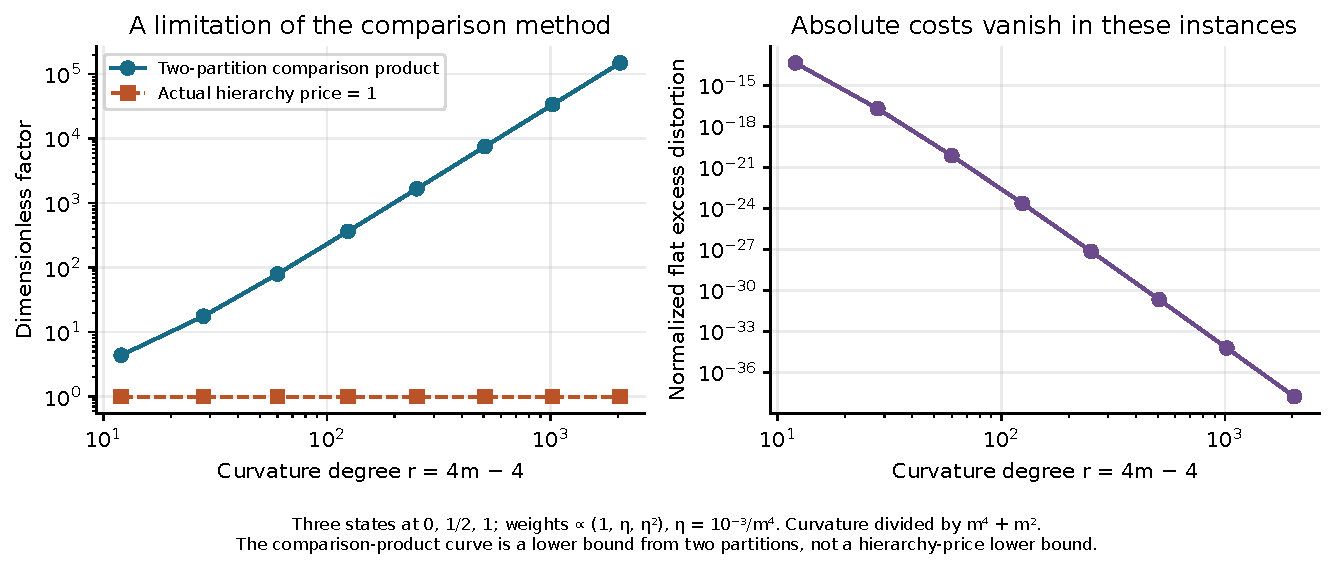
\includegraphics[width=\textwidth]{coordinate_method_obstruction.pdf}
\caption{The same finite examples: the two-partition comparison product
grows while the actual hierarchy price stays one (left), and the
normalized flat distortion becomes very small (right). Lines connect
computed points; no asymptotic fit is used.}
\label{fig:coordinate-check}
\end{figure}


\paragraph{Exact finite indicator-oracle checks.}
The script \texttt{check\_indicator\_bridge.py} uses exact rational
arithmetic for 27 finite populations. All 108 population-oracle states,
81 birth/refit transitions, and 27 unrestricted one-unit Bayes fits pass
their identity checks. The birth-only example retains excess risk $1/16$
after copying the old report, while the new flat optimum is zero, exactly
as in Proposition~\ref{prop:p9-nontransfer}. These computations evaluate
known population posteriors and algebraic refits; they are not training
or generalization experiments.

\paragraph{Reproducibility and evidence boundary.}
The source bundle includes the scripts, JSON results, execution logs,
environment details, and input hashes under
\texttt{research/experiments} and \texttt{research/prior\_art}.
Every experiment uses finite calculations on the stated examples.
The explicit lower proof and the upper proof do not depend on the
computational checks. No external training run, package installation,
or modification of an earlier research phase is needed to read or build
this paper.


\section{Remaining questions and interpretation}
Theorem~\ref{thm:weighted-sharp} and Appendix~\ref{sec:ext-weights} settle
the arbitrary-positive-weight four-state degree order. They rule out an
$\Omega(r^2)$ construction in this exact domain, whether based on
Chebyshev needles, Jacobi kernels, or another nonnegative polynomial.
They do not rule out that order for more source states or different
capacity pairs. Both the arbitrary-source-count two-capacity order and
the arbitrary-source-count all-capacity order in Table~\ref{tab:scope}
remain unresolved.

The coordinate example has a different implication. Its two-sided
comparison condition factor is already $\Omega(r^2\log r)$ after choosing
the best constants for a single generator and source, while the source's
hierarchy price is exactly one. Thus improving a proof based only on
that global partition comparison requires extra structure or a different
coordinate. The example is no lower bound on the price of optimal
hierarchies and does not prove necessity of the logarithm in the
general all-capacity upper bound.

The restricted neural model is similarly exact but narrow: it identifies
population oracle costs when hidden units are indicators of a partition,
arbitrary subset splits are allowed, and reports are refit exactly.
Removing those restrictions changes the flat oracle class. No SGD,
Adam, finite-sample, continuous-domain, computational-efficiency, or
generalization result is deduced. Finally, the bounded-loss lower witnesses
have vanishing flat excess risks. Large multiplicative prices therefore
do not establish a nonvanishing absolute-risk penalty.

\paragraph{Review and provenance.}
The upper theorem, its weighted kernel inequalities, and all displayed
constants received an independent internal mathematical review. The
coordinate obstruction and the two bridge/asymmetry notes also received
independent internal checks. The source bundle records the exact reviewed
file hashes and the arithmetic evidence. Classical approximation tools and
prior Phase~8 arguments are identified explicitly; the appendix lower
construction is reproduced with attribution. The focused source ledger
documents access limits: original Kro\'o sources in the needle attribution
chain were not read in this pass, and the earlier original-Lin access
limitation remains. These checks establish neither external peer review
nor historical priority.

\appendix
\section{The matching endpoint lower construction}
\label{sec:ext-weights}
This appendix reproduces the Phase~8 endpoint construction~\cite{huang8},
with its full kernel proof and bounded-loss normalization. Combined with
Theorem~\ref{thm:weighted-sharp}, it proves the matching sharp lower order.
The source weights and posterior gaps are both allowed to vary with degree.

\subsection{An endpoint-localized polynomial curvature}
The only approximation ingredient needed is elementary external growth of
Chebyshev polynomials. It is a classical polynomial localization mechanism;
the identity $T_n(\cosh v)=\cosh(nv)$ is recorded in
\cite[Eq.~18.5.1]{dlmf}. Squared-Chebyshev endpoint needles and their exponential tail mechanisms
also appear explicitly in Slot--Laurent~\cite[Section~4.1]{slot2019};
see also~\cite{slot2020}. None of this polynomial technology is claimed
as original here. The kernel estimates below are supplied in full.

For an integer $n$ sufficiently large, put
\begin{equation}
 d=d_n=\left(\frac{4\log n}{n}\right)^2,\qquad
 p_n(t)=T_n\!\left(\frac{2t-1-d}{1-d}\right)^2,\qquad
 Z_n=\int_0^1p_n(t)\rd t,\qquad
 \kappa_n(t)=\frac{p_n(t)}{Z_n}.
 \label{eq:ext-endpointneedle}
\end{equation}
Here $\kappa_n$ denotes its polynomial on the whole real line, although its
normalization and probability-mass estimates refer only to $[0,1]$.
Its degree is $2n$ and it is nonnegative everywhere. For $t\in[d,1]$ the
argument of $T_n$ belongs to $[-1,1]$, so $p_n(t)\le1$. On $[0,d/2]$ the
absolute value of that argument is at least $1+d/(1-d)\ge1+d$.
For $0\le v\le1$, $\operatorname{arcosh}(1+v)\ge\sqrt v$: for example,
$\cosh(\sqrt v)\le1+v$ follows by its power series. Using the parity of
$T_n$ and the hyperbolic identity therefore gives, for $d\le1/4$,
\[
 p_n(t)\ge\tfrac14e^{2n\sqrt d}\quad(0\le t\le d/2),\qquad
 Z_n\ge\frac d8 e^{2n\sqrt d}.
\]
Consequently
\begin{equation}
 \int_d^1\kappa_n(t)\rd t\le\tau_n,
 \qquad
 \tau_n:=8d^{-1}e^{-2n\sqrt d}
       =\frac{1}{2n^6(\log n)^2}=o(d^3).
 \label{eq:ext-tail}
\end{equation}
The normalized maximum also satisfies
\begin{equation}
 \max_{[0,1]}\kappa_n\le32n^2.
 \label{eq:ext-max}
\end{equation}
For completeness, the rescaled classical Markov inequality
\cite{shadrin} gives $\|\kappa_n'\|_\infty\le2(2n)^2M$ when
$M=\|\kappa_n\|_\infty$. From a maximizer, one direction remains in $[0,1]$
for length $1/(4(2n)^2)$, throughout which $\kappa_n\ge M/2$.
Integrating and using $\int_0^1\kappa_n=1$ yields $M\le8(2n)^2$.

Define
\begin{equation}
 g_n(t)=\kappa_n(t)+\kappa_n(1-t)+d^2,
 \qquad \ph_n''=g_n,
 \qquad \ph_n'(1/2)=\ph_n(1/2)=0.
 \label{eq:ext-curvature}
\end{equation}
This curvature is strictly positive on the whole real line and symmetric
about $1/2$. Its degree is exactly $r=2n$: both squared-polynomial terms
have positive leading coefficient of the same even degree. The generator
is a symmetric strictly convex polynomial of degree $2n+2$.

\subsection{All deterministic hierarchies are expensive}
Take the sorted source locations and probabilities
\begin{equation}
 (x_A,x_B,x_C,x_D)=(0,2d,1-2d,1),\qquad
 (p_A,p_B,p_C,p_D)=(a,b,b,a),\qquad
 b=d^2,\quad a=\tfrac12-b.
 \label{eq:ext-source}
\end{equation}
For all sufficiently large $n$, these are distinct and all weights are
positive. Every distortion and flat denominator below uses these original
weights, with no conditional renormalization of a cell.

For a pair $u<v$ of respective weights $p_u,p_v$, its exact Jensen curvature
kernel is
\begin{equation}
 K_{uv}(t)=\min\{p_u(t-u),p_v(v-t)\}\,
           \mathbf1_{[u,v]}(t).
 \label{eq:ext-pairkernel}
\end{equation}
For an arbitrary cell $S$, the kernel is
\[
 K_S(t)=\sum_{i\in S}p_i(x_i-t)_+-p_S(m_S-t)_+,
 \qquad D(S)=\int K_S(t)g_n(t)\rd t.
\]
These formulas follow by writing a twice differentiable convex generator,
up to an affine term, as an integral of $(x-t)_+$ against its curvature.

Set
\[
 P=D(AB)=D(CD),\quad q=D(BC),\quad
 T=D(ABC)=D(BCD),\quad J=D(AD).
\]
The equalities use reflection symmetry. Since
$128n^2b=128n^2d^2\to0$, equations
\eqref{eq:ext-tail}--\eqref{eq:ext-max} imply, eventually,
\begin{equation}
 I=[4b,d]\ne\varnothing,\qquad
 \int_I\kappa_n(t)\rd t
 \ge1-\tau_n-128n^2b\ge\tfrac12.
 \label{eq:ext-core}
\end{equation}
We may also assume $d\le1/16$ and $\tau_n\le d^2/2$.

The pair $AB$ has mean $4bd$. Thus on $I$, which lies above that mean,
$K_{AB}(t)=b(2d-t)\ge bd$. Conversely $K_{AB}\le2bd$ everywhere.
On $[0,2d]$, the reflected needle contributes at most $\tau_n$ to the
integrated curvature, since $1-2d\ge d$. Hence
\[
 \int_0^{2d}g_n\le1+\tau_n+2d^3\le2.
\]
Together with \eqref{eq:ext-core}, this proves
\begin{equation}
 \frac{bd}{2}\le P\le4bd.
 \label{eq:ext-nearpair}
\end{equation}
For the middle pair, $K_{BC}\le b/2$. The two needles contribute at most
$2\tau_n$ on $[2d,1-2d]$, and the constant curvature contributes at most
$d^2$. Therefore
\begin{equation}
 0<q\le\frac b2(2\tau_n+d^2)\le bd^2.
 \label{eq:ext-middlepair}
\end{equation}
The triple $ABC$ has mean $b/(1/2+b)\le2b$. For $t\in I$ this mean lies
below $t$, while both inner locations lie above $t$, so
\[
 K_{ABC}(t)=b(2d-t)+b(1-2d-t)=b(1-2t)\ge b/2.
\]
The outer pair has kernel $K_{AD}(t)=a\min(t,1-t)$. On $I$ this is at
least $4ab\ge b$, because $a\ge1/4$. Thus
\begin{equation}
 T\ge b/4,\qquad J\ge b/2.
 \label{eq:ext-coarse}
\end{equation}

We now cover all deterministic hierarchy choices, including noncontiguous
ones. A hierarchy with fewer than the allowed numbers of cells can be
refined to exactly three fine cells and two coarse cells without increasing
either cost: split fine cells within their current coarse cells, then split
the coarse level if necessary by grouping the three fine cells. Every exact
three-cell partition of four states merges one pair. Besides $BC$, each
pair has cost at least $P$. This is immediate for $AB,CD$; the pair $AC$
has the same endpoint weights as $AB$ and a more distant right endpoint,
so its kernel dominates $K_{AB}$ pointwise, and $BD$ is its reflection.
Finally, $J\ge b/2\ge P$ by \eqref{eq:ext-nearpair} and $d\le1/16$.

If the fine pair is not $BC$, then $\OPT_3\le q$ gives fine-level ratio
at least $P/q\ge1/(2d)$. If the fine pair is $BC$, its exact two-cell
coarsenings are $ABC\mid D$, $A\mid BCD$, and $AD\mid BC$. By
\eqref{eq:ext-coarse} each costs at least $b/4$. Since the available
coarse split $AB\mid CD$ gives $\OPT_2\le2P\le8bd$, this hierarchy has
coarse-level ratio at least $1/(32d)$. These two cases prove
\begin{equation}
 \rho_{\ph_n,\detp}\ge\frac1{32d_n},\qquad
 \rho_{\ph_n,\stp}\ge\frac1{64d_n},
 \label{eq:ext-lower}
\end{equation}
the second inequality following from Lemma~\ref{lem:ext-rounding}.
Notice that this proof needs neither exact flat optimizer identification nor
an assertion that contiguous deterministic hierarchies exhaust the optimum.

\begin{theorem}[Matching arbitrary-weight four-state lower bound]
\label{thm:ext-weightdegenerate}
Let $\widehat C_r^{\detp}$ and $\widehat C_r^{\stp}$ denote the two/three-output
four-state degree envelopes in which all positive source weights are allowed.
There is an absolute $c>0$ such that, for all sufficiently large $r$,
\[
 \widehat C_r^{\detp}\ge\widehat C_r^{\stp}
 \ge c\frac{r^2}{(\log r)^2}.
\]
Consequently no absolute-constant $O(r/\log r)$ bound holds in this weighted
four-state setting. The witnesses can have all posteriors in $[1/4,3/4]$
and polynomial generators inducing smooth strictly proper losses bounded
in $[0,1/2]$.
\end{theorem}
\begin{proof}
Equations \eqref{eq:ext-endpointneedle} and \eqref{eq:ext-lower} give the
claim at degrees $r=2n$, since $1/d_n=n^2/(16(\log n)^2)$.
For a degree-at-most-$r$ envelope take $n=\lfloor r/2\rfloor$.

To put all posteriors in the stated interior interval, use
$y=1/4+x/2$. The four locations become
$(1/4,1/4+d,3/4-d,3/4)$.
Let $M_n=\max_{t\in[-1/2,3/2]}g_n(t)$ and set
\[
 \widetilde\ph_n(y)=\frac{\ph_n(2y-1/2)}{4M_n}.
\]
The fact that $g_n$ is a sum of squares plus $d^2$ on the \emph{whole real
line} ensures $0<\widetilde\ph_n''\le1$ on $[0,1]$. This affine coordinate
change and positive rescaling preserve every price and curvature degree.
The generator remains symmetric about $1/2$. Put
$h(y)=\widetilde\ph_n(0)-\widetilde\ph_n(y)$ and define
\[
 \ell(y,1)=h(y)+(1-y)h'(y),\qquad
 \ell(y,0)=h(y)-yh'(y).
\]
Expected regret is $B_{\widetilde\ph_n}$, so the loss is strictly proper.
Symmetry and the supporting-line inequalities make both losses nonnegative;
their derivatives are $-(1-y)\widetilde\ph_n''(y)$ and
$y\widetilde\ph_n''(y)$, respectively. Their common maximum is
$\widetilde\ph_n'(1)=-\widetilde\ph_n'(0)
=\int_{1/2}^1\widetilde\ph_n''\le1/2$.
\end{proof}


The smallest mass in this family is $d_n^2=256(\log n)^4/n^4$.
The generators, weights, and posterior gaps all vary with $n$. This does
not determine a sharp joint minimum-mass/degree envelope. The normalization
preserves price, not absolute excess cost; explicit vanishing flat-cost
bounds appear after Theorem~\ref{thm:weighted-sharp}.

\section{Exact endpoint moments and polynomial Bregman asymmetry}
\label{sec:p9-exact-asymmetry}

The endpoint first-moment problem can be solved exactly by positive
quadrature. Its sum-of-squares version is already the linear-objective
case in de Klerk--Laurent, \emph{Worst-case examples for Lasserre's
measure--based hierarchy for polynomial optimization on the hypercube},
\cite[Theorem~3.1 and Corollary~3.2]{deklerk}. The reduction below is a
classical quadrature consequence, not a new approximation principle.
It strengthens the constants and identifies extremizers for one ingredient;
it does not determine a hierarchy price.

For an integer $r\ge0$, define
\[
 \lambda_r=\inf_{\substack{g\not\equiv0,\ \deg g\le r\\
                                      g\ge0\text{ on }[0,1]}}
       \frac{\int_0^1 t g(t)\,dt}{\int_0^1g(t)\,dt}.
\]
For $\alpha,\beta>-1$, write $\xi_j^{(\alpha,\beta)}$ for the
smallest zero of the degree-$j$ Jacobi polynomial
$P_j^{(\alpha,\beta)}$ on $[-1,1]$, with weight
$(1-x)^\alpha(1+x)^\beta$.

\begin{theorem}[Exact endpoint moment]
For every $m\ge0$,
\begin{equation}
 \lambda_{2m}=\frac{1+\xi_{m+1}^{(0,0)}}2,
 \qquad
 \lambda_{2m+1}=\frac{1+\xi_{m+1}^{(1,0)}}2.
 \label{eq:p9-exact-lambda}
\end{equation}
The infima are attained. In particular,
$\lambda_r=\Theta((r+1)^{-2})$.
\end{theorem}
\begin{proof}
For even degree, take the $m+1$-node Gauss--Legendre rule on $[0,1]$
\cite[Section~3.5(v)]{dlmf}.
Its nodes $t_1<\cdots<t_{m+1}$ are the shifted Legendre zeros, its
weights $\omega_j$ are positive, and it integrates polynomials of degree
at most $2m+1$ exactly. Thus for every admissible $g$,
\[
 \int_0^1 t g(t)\,dt-t_1\int_0^1g(t)\,dt
  =\sum_{j=1}^{m+1}\omega_j(t_j-t_1)g(t_j)\ge0.
\]
The polynomial $g(t)=\prod_{j=2}^{m+1}(t-t_j)^2$ has degree $2m$,
is nonnegative, and makes the right side zero. The empty product for
$m=0$ is one. This proves the first formula.

For clarity, the requisite odd-degree quadrature rule is constructed here.
Let $J$ be the degree-$m+1$ polynomial orthogonal for weight $1-t$ on
$[0,1]$. Its $m+1$ simple interior zeros are $t_1<\cdots<t_{m+1}$;
add the node $t_{m+2}=1$. Integrate the Lagrange interpolant on these
$m+2$ nodes to define an interpolatory rule. For a polynomial $f$ of
degree at most $2m+2$, divide
\[
 f(t)=(t-1)J(t)q(t)+s(t),\qquad
 \deg q\le m,\quad\deg s\le m+1.
\]
The first summand integrates to zero by orthogonality and vanishes at all
nodes. The rule therefore integrates $f$ exactly. If $L_j$ is the
degree-$m+1$ cardinal Lagrange polynomial, exactness for $L_j^2$ gives
$\omega_j=\int_0^1L_j(t)^2\,dt>0$.
Applying this positive rule to $g$ and $tg$ proves that the moment ratio
is at least $t_1$. Equality is attained by
\[
 g(t)=(1-t)\prod_{j=2}^{m+1}(t-t_j)^2,
\]
of degree $2m+1$. The orthogonality weight identifies $J$ with the
shifted $P_{m+1}^{(1,0)}$, proving the second formula.

For both fixed parameter pairs, the smallest Jacobi zero is
$-1+\Theta((m+1)^{-2})$. This standard extreme-zero estimate is recorded
in de Klerk--Laurent~\cite[Corollary~2.3]{deklerk}, and gives the stated order.
\end{proof}

\begin{theorem}[Sharp oriented polynomial asymmetry]
Let $\varphi''=g$ be a nonnegative nonzero polynomial of degree at most
$r$ on an interval $[u,v]$, $u<v$. Then
\begin{equation}
 \max\left\{\frac{B_\varphi(v,u)}{B_\varphi(u,v)},
             \frac{B_\varphi(u,v)}{B_\varphi(v,u)}\right\}
 \le\frac{1-\lambda_r}{\lambda_r}.
 \label{eq:p9-exact-asymmetry}
\end{equation}
The bound is attained within nonnegative polynomial curvature, is the
supremum if curvature is required to be strictly positive everywhere on
the interval, and is $\Theta((r+1)^2)$.
\end{theorem}
\begin{proof}
Affine rescaling reduces to $[0,1]$. Writing
$\mu=\int_0^1g$ and $a=\mu^{-1}\int_0^1tg$ gives
\[
 B_\varphi(0,1)=a\mu,
 \qquad B_\varphi(1,0)=(1-a)\mu.
\]
The preceding theorem and its reflected version imply
$\lambda_r\le a\le1-\lambda_r$. The ratio bound follows, and the
extremizing curvatures above attain equality. Such curvature still
induces strict convexity because it vanishes on no nonempty interval.
For everywhere-positive curvature, add $\varepsilon>0$ and send it to
zero; all displayed integrals converge and the denominator stays positive.
The extreme-zero order proves the last assertion.
\end{proof}

\paragraph{Why oriented asymmetry is not a hierarchy lower bound.}
After normalizing $\int_0^1g=1$, a first-moment estimate
$\int_0^1tg=O(r^{-2})$ gives only
$\int_d^1g\le O((r^2d)^{-1})$. At $d\asymp r^{-2}$ this is a
constant bound, whereas the existing four-state endpoint proof uses a
leakage bound much smaller than a power of $d$. The exact moment theorem
does not supply that stronger assertion. Conversely, sharp oriented
asymmetry need not generate incompatible optimal partitions at two
capacities. It cannot be substituted for a hierarchy-price lower bound.
The general-source $O(r^2)$ two-capacity bound in Phase~8 uses an anchor
quasi-triangle inequality, a different optimization from the endpoint
orientation ratio solved here. The sharp four-state result in
Theorem~\ref{thm:weighted-sharp} instead uses a direct kernel argument.

\begin{thebibliography}{99}
\bibitem{arutyunova}
Anna Arutyunova and Heiko R\"oglin.
The price of hierarchical clustering.
\emph{Algorithmica} 87 (2025), 1420--1452.
\url{https://doi.org/10.1007/s00453-025-01327-7}.

\bibitem{banerjee}
Arindam Banerjee, Srujana Merugu, Inderjit S. Dhillon, and Joydeep Ghosh.
Clustering with Bregman divergences.
\emph{Journal of Machine Learning Research} 6 (2005), 1705--1749.
\url{https://www.jmlr.org/papers/v6/banerjee05b.html}.

\bibitem{deklerk}
Etienne de Klerk and Monique Laurent.
Worst-case examples for Lasserre's measure-based hierarchy for polynomial
optimization on the hypercube.
\emph{Mathematics of Operations Research} 45(1) (2020), 86--98.
\url{https://arxiv.org/abs/1804.05524}.

\bibitem{gneiting}
Tilmann Gneiting and Adrian E. Raftery.
Strictly proper scoring rules, prediction, and estimation.
\emph{Journal of the American Statistical Association} 102(477) (2007),
359--378. \url{https://doi.org/10.1198/016214506000001437}.

\bibitem{gomes}
Erika Gomes-Gon\c calves, Henryk Gzyl, and Frank Nielsen.
\emph{Geometry and Clustering with Metrics Derived from Separable Bregman
Divergences}. Preprint, 2018.
\url{https://arxiv.org/abs/1810.10770}.

\bibitem{gzyl}
Henryk Gzyl.
\emph{From Generalized Arithmetic Means to Geodesics to Hamilton Dynamics
to Bregman Divergences}. Preprint, 2020.
\url{https://arxiv.org/abs/2007.15473}.

\bibitem{huang8}
Wenyu Huang.
\emph{Polynomial Curvature and Weight Dependence in Optimal Cardinality
Hierarchies}. Phase~8 v2 working paper, University of California San Diego,
7 October 2026. Prior project manuscript; source and review bundle retained
with this follow-up's project archive.

\bibitem{lasserre}
Jean B. Lasserre.
\emph{Connecting Optimization with Spectral Analysis of Tri-diagonal
Matrices}. Preprint, 2019.
\url{https://arxiv.org/abs/1907.09784}.

\bibitem{lin}
Guolong Lin, Chandrashekhar Nagarajan, Rajmohan Rajaraman, and David P. Williamson.
A general approach for incremental approximation and hierarchical clustering.
\emph{SIAM Journal on Computing} 39(8) (2010), 3633--3669.
\url{https://doi.org/10.1137/070698257}.

\bibitem{dlmf}
National Institute of Standards and Technology.
\emph{Digital Library of Mathematical Functions}.
Sections 3.5(v) (Gaussian quadrature), 18.5 (representations), and 18.16
(zeros). \url{https://dlmf.nist.gov/3.5#v};
\url{https://dlmf.nist.gov/18.5}; \url{https://dlmf.nist.gov/18.16}.

\bibitem{reid}
Mark D. Reid and Robert C. Williamson.
Information, divergence and risk for binary experiments.
\emph{Journal of Machine Learning Research} 12 (2011), 731--817.
\url{https://www.jmlr.org/papers/v12/reid11a.html}.

\bibitem{shadrin}
A. Shadrin.
\emph{Twelve Proofs of the Markov Inequality}. Author-hosted exposition.
\url{https://www.damtp.cam.ac.uk/user/na/people/Alexei/papers/markov.pdf}.

\bibitem{slot2019}
Lucas Slot and Monique Laurent.
\emph{Improved Convergence Analysis of Lasserre's Measure-based Upper Bounds
for Polynomial Minimization on Compact Sets}. Preprint, 2019.
Section~4.1, Definition~5, Theorem~12, and subsequent tail estimates.
\url{https://arxiv.org/abs/1905.08142}.

\bibitem{slot2020}
Lucas Slot and Monique Laurent.
Near-optimal analysis of univariate moment bounds for polynomial optimization.
\emph{Mathematical Programming} 188 (2021), 443--460.
Preprint title: \emph{Near-optimal analysis of Lasserre's univariate
measure-based bounds for multivariate polynomial optimization}.
\url{https://arxiv.org/abs/2001.11289}.
\end{thebibliography}

\end{document}
